\documentclass[24pt, a0paper, portrait, margin=5mm, innermargin=5mm,
               blockverticalspace=10mm, blocktitlewidthratio=0.5, colspace=10mm, 
               subcolspace=10mm]{tikzposter} 

% Change font     
\renewcommand{\familydefault}{\sfdefault}

% LATEX PACKAGES
% --------------
  
\usepackage{graphicx}  % package for inserting images, including .pdf
\usepackage{adjustbox} % package for cropping images
% \usepackage[colorlinks=true, urlcolor=red]{hyperref} % package for url and hyperlinks
\usepackage{wrapfig}
\usepackage{lmodern} %mix italic and bold
\usepackage{hyperref}% for url
\usepackage{authblk}
\usepackage{graphicx} 
\usepackage{caption}
\usepackage{mwe}
\usepackage[absolute]{textpos}
\usepackage{selinput}
\usepackage{multicol}
\usepackage{tikz}

% \usepackage{anyfontsize} %increase overall font size
\SelectInputMappings{%
  Lcaron={Ľ}
}

\definecolor{calpolypomonagreen}{rgb}{0.12, 0.3, 0.17}

% TITLE, AUTHORS, INSTITUTE
% -------------------------

\title{\textbf{\parbox{\linewidth}{\centering Reduced \textit{Eimeria} and pinworms loads in hybrid mice of the European house mouse hybrid zone}}}

\author[1,2]{\Large Alice~Balard}
\author[1,2]{Victor~Hugo~Jarqu\'{i}n-D\'{i}az}
\author[1]{Jenny~Jost}
\author[3]{Iva~Martincov\'{a}}
\author[3]{{Ľ}udov\'{i}t \v{D}ureje}
\author[3]{Jaroslav~Pi\`alek}
\author[4]{Milo\v{s}~Macholán}
\author[3]{Jo\"{e}lle~Go\"{u}y~de~Bellocq}
\author[3]{Stuart~J.E.~Baird}
\author[1,2]{Emanuel~Heitlinger}

\affil[1]{\large Institute for Biology. Department of Molecular Parasitology. Humboldt University Berlin, Germany}
\affil[2]{\large Leibniz Institute for Zoo and Wildlife Research, Berlin, Germany}
\affil[3]{\large Research Facility Studenec, Institute of Vertebrate Biology, Czech Academy of Sciences, Czech Republic}
\affil[4]{\large Laboratory of Mammalian Evolutionary Genetics, Institute of Animal Physiology and Genetics, Czech Academy of Sciences, Czech Republic\vspace{-4ex}% reduce space
}

\makeatletter
\def\maketitle{\AB@maketitle}
\makeatother

% THEME SETTING
% -------------
\usetheme{Simple}

\colorlet{titlebgcolor}{calpolypomonagreen}
\colorlet{blocktitlefgcolor}{calpolypomonagreen}


% HEAD
% ----

\begin{document}
\maketitle

% Context
% ----

\block{General}
{
	\begin{itemize}
	   \item Parasite models: 
	    \begin{itemize}
	  		\item \textit{Eimeria} spp., obligate intracellular parasite (Apicomplexa: Coccidia). \textbf{High impact on host health expected}
	  		\item Pinworms (\textit{Aspiruluris tetraptera} and \textit{Syphacia obvelata}). \textbf{Low impact on host health expected}
	    \end{itemize}
	  \item Host model: \textit{Mus musculus domesticus}, \textit{M. m. musculus} and their hybrids	
	  \item Aim of the study: \textbf{Investigating hybrid susceptibility/resistance of house mice to parasites presenting different pathogenicity, using prevalence and intensity data in a new transect of the European house mouse hybrid zone}
  \end{itemize}
}	

% MATANDMET
% ----

% playing with multicolumn text
\block{Material \& Methods}{
  \begin{multicols*}{2}
    \begin{itemize}
 \item Sampling 660 mice over 4 years; Host genotyping (4-14 diagnostic markers) on a 0 to 1 scale (equal admixture hybrids = 0.5)
 \item \textit{Eimeria} load estimated by quantitative PCR 
 \item Pinworm load estimated by count
 \item Modellisation of parasite load along hybridization index, test hybrid effect by maximum likelihood 
 \item Logistic regression presence/absence of parasite in direction of the hybrid zone center
 \item Body condition = residuals body length/body weight. Modellisation of body condition along hybridization index, test hybrid effect by maximum likelihood, test difference between infected/non-infected 
      \end{itemize}
    \begin{tikzfigure}[]
               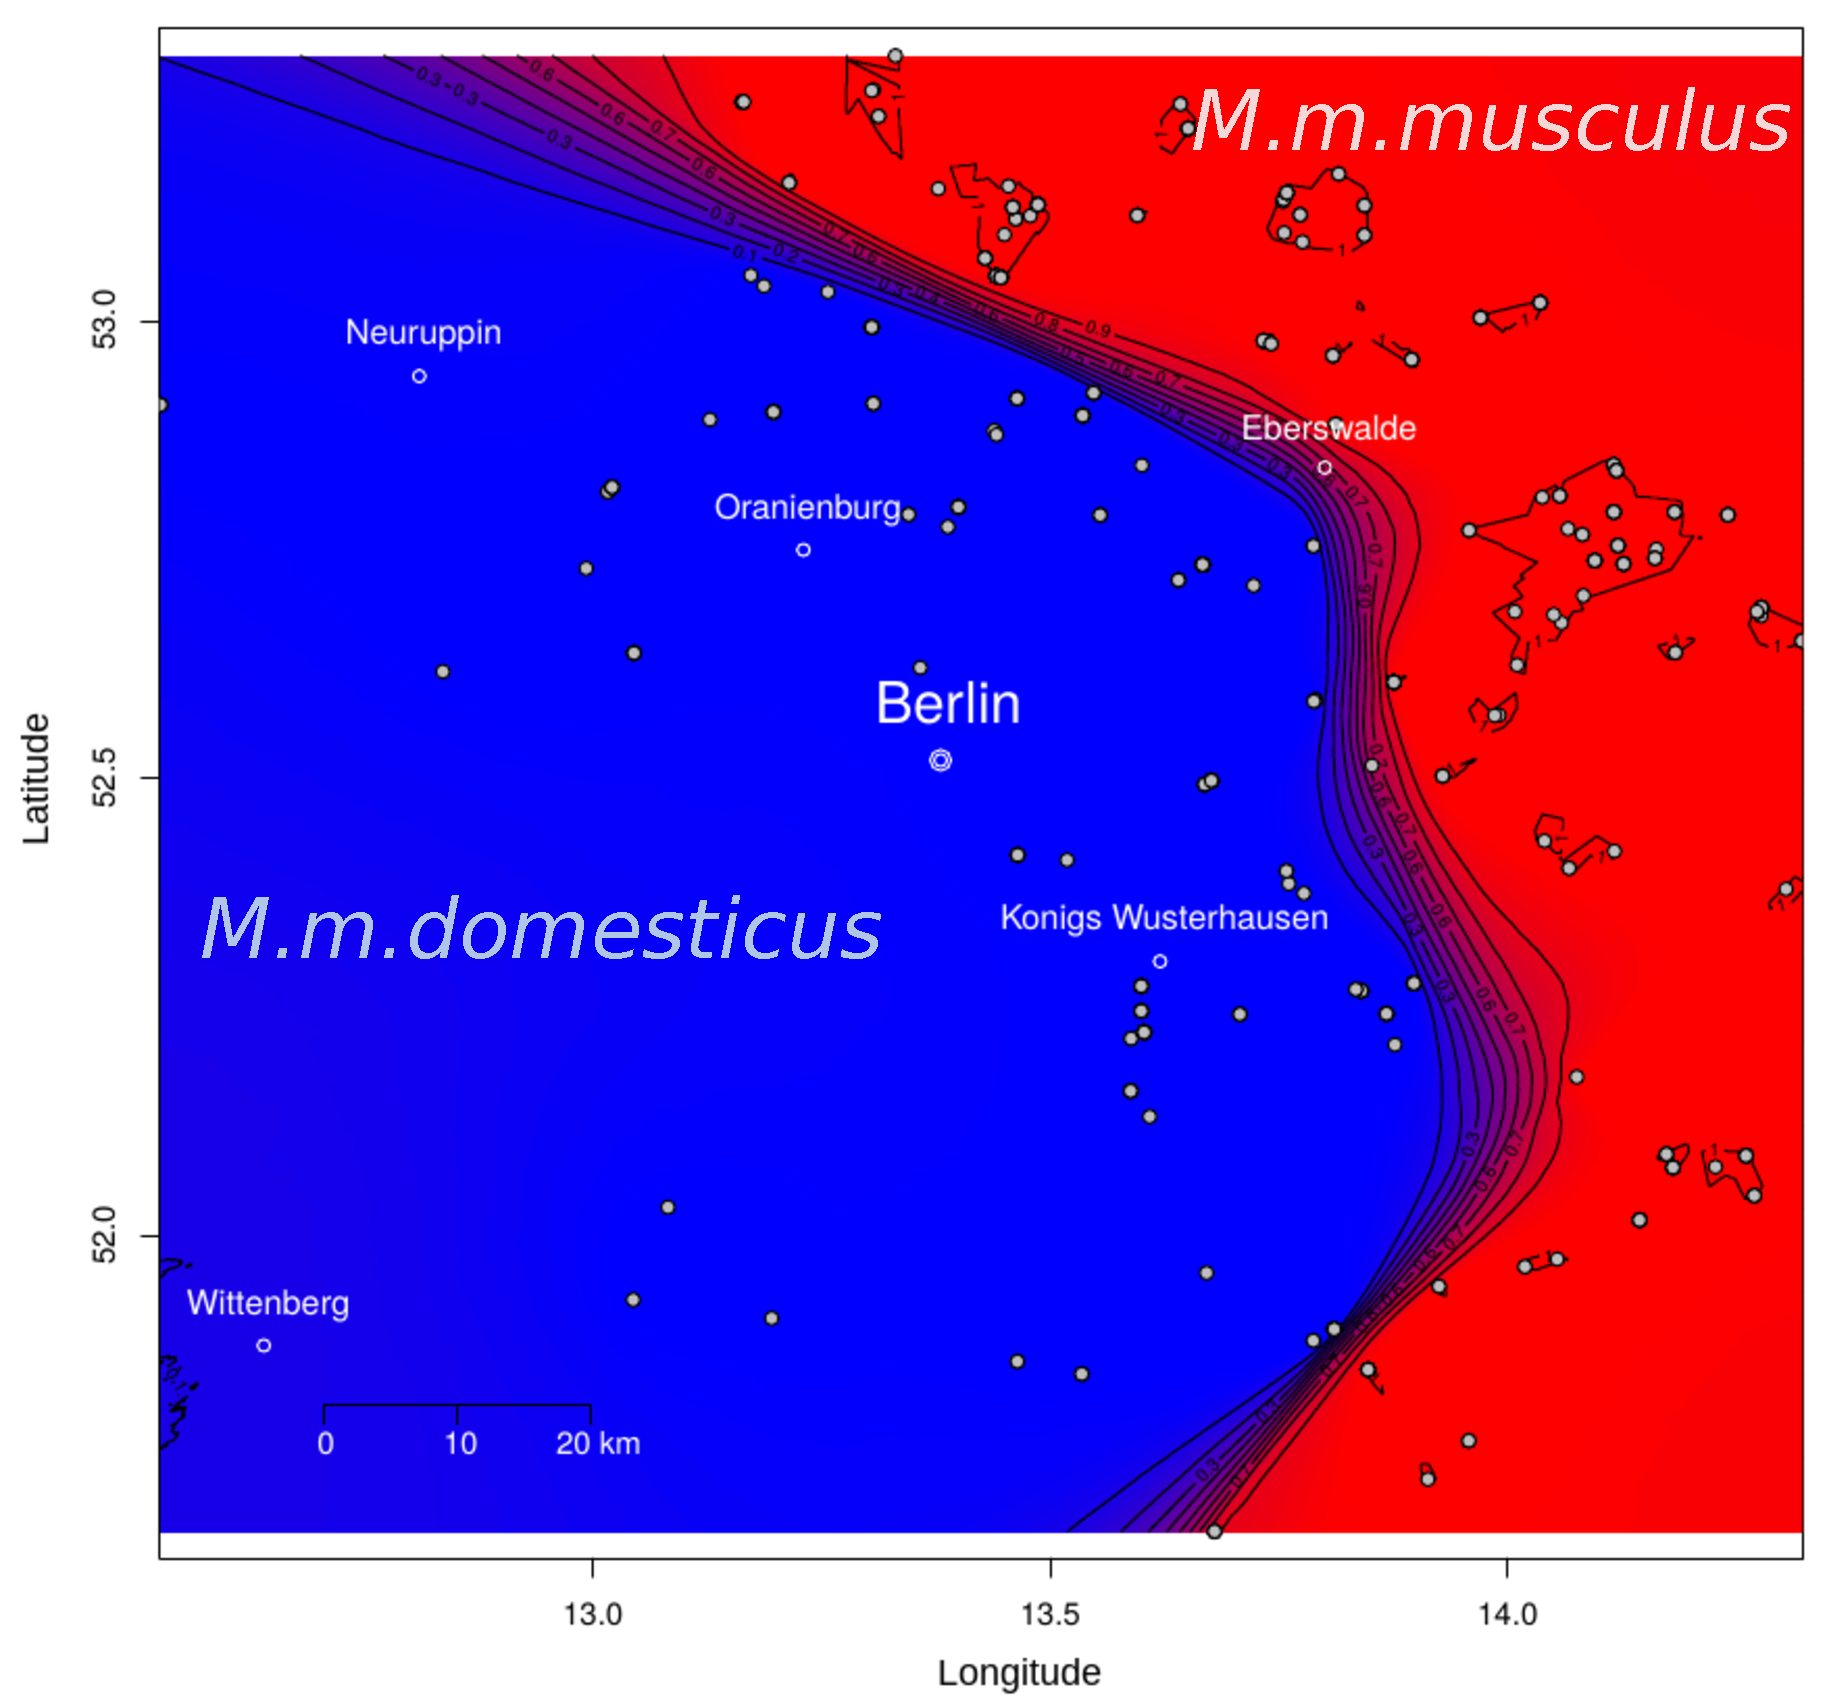
\includegraphics[scale=0.5]{Figure1.pdf}
    \end{tikzfigure}
    \end{multicols*}
}

% Results: parasite load
% -------

\block{Results: \textit{Eimeria} spp. and pinworm load lower in hybrids than in parental mice}
      {
      \begin{multicols*}{2}
      
      \begin{multicols*}{2}
\Large \centering \textit{Eimeria}
      \begin{tikzfigure}[]
        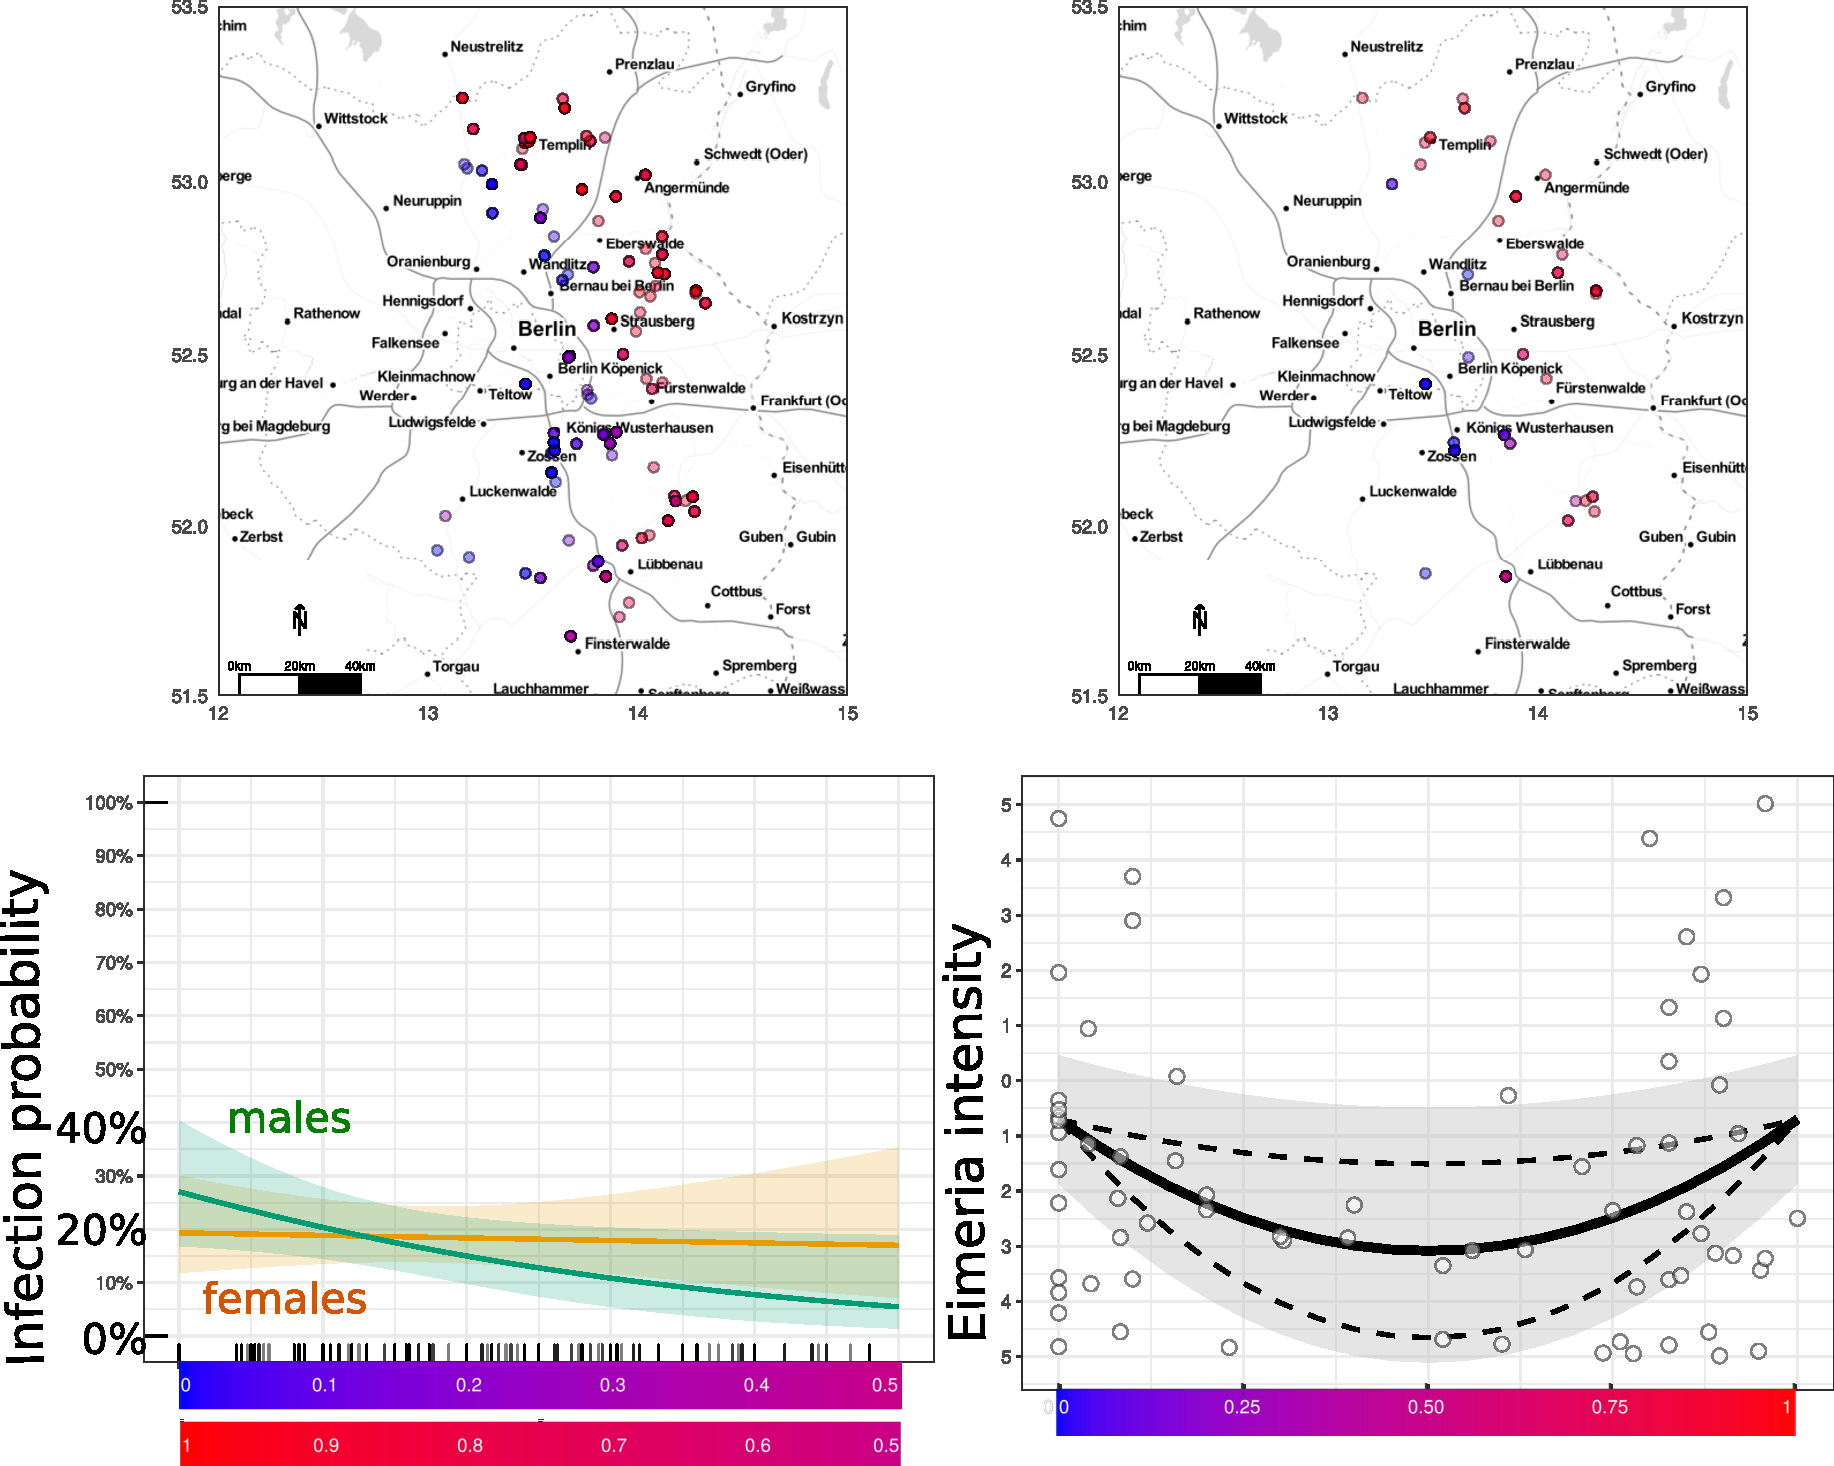
\includegraphics[scale=0.7]{Figure2.pdf}
      \end{tikzfigure} \vfill\null \columnbreak


\Large \centering Pinworms
      \begin{tikzfigure}[]
        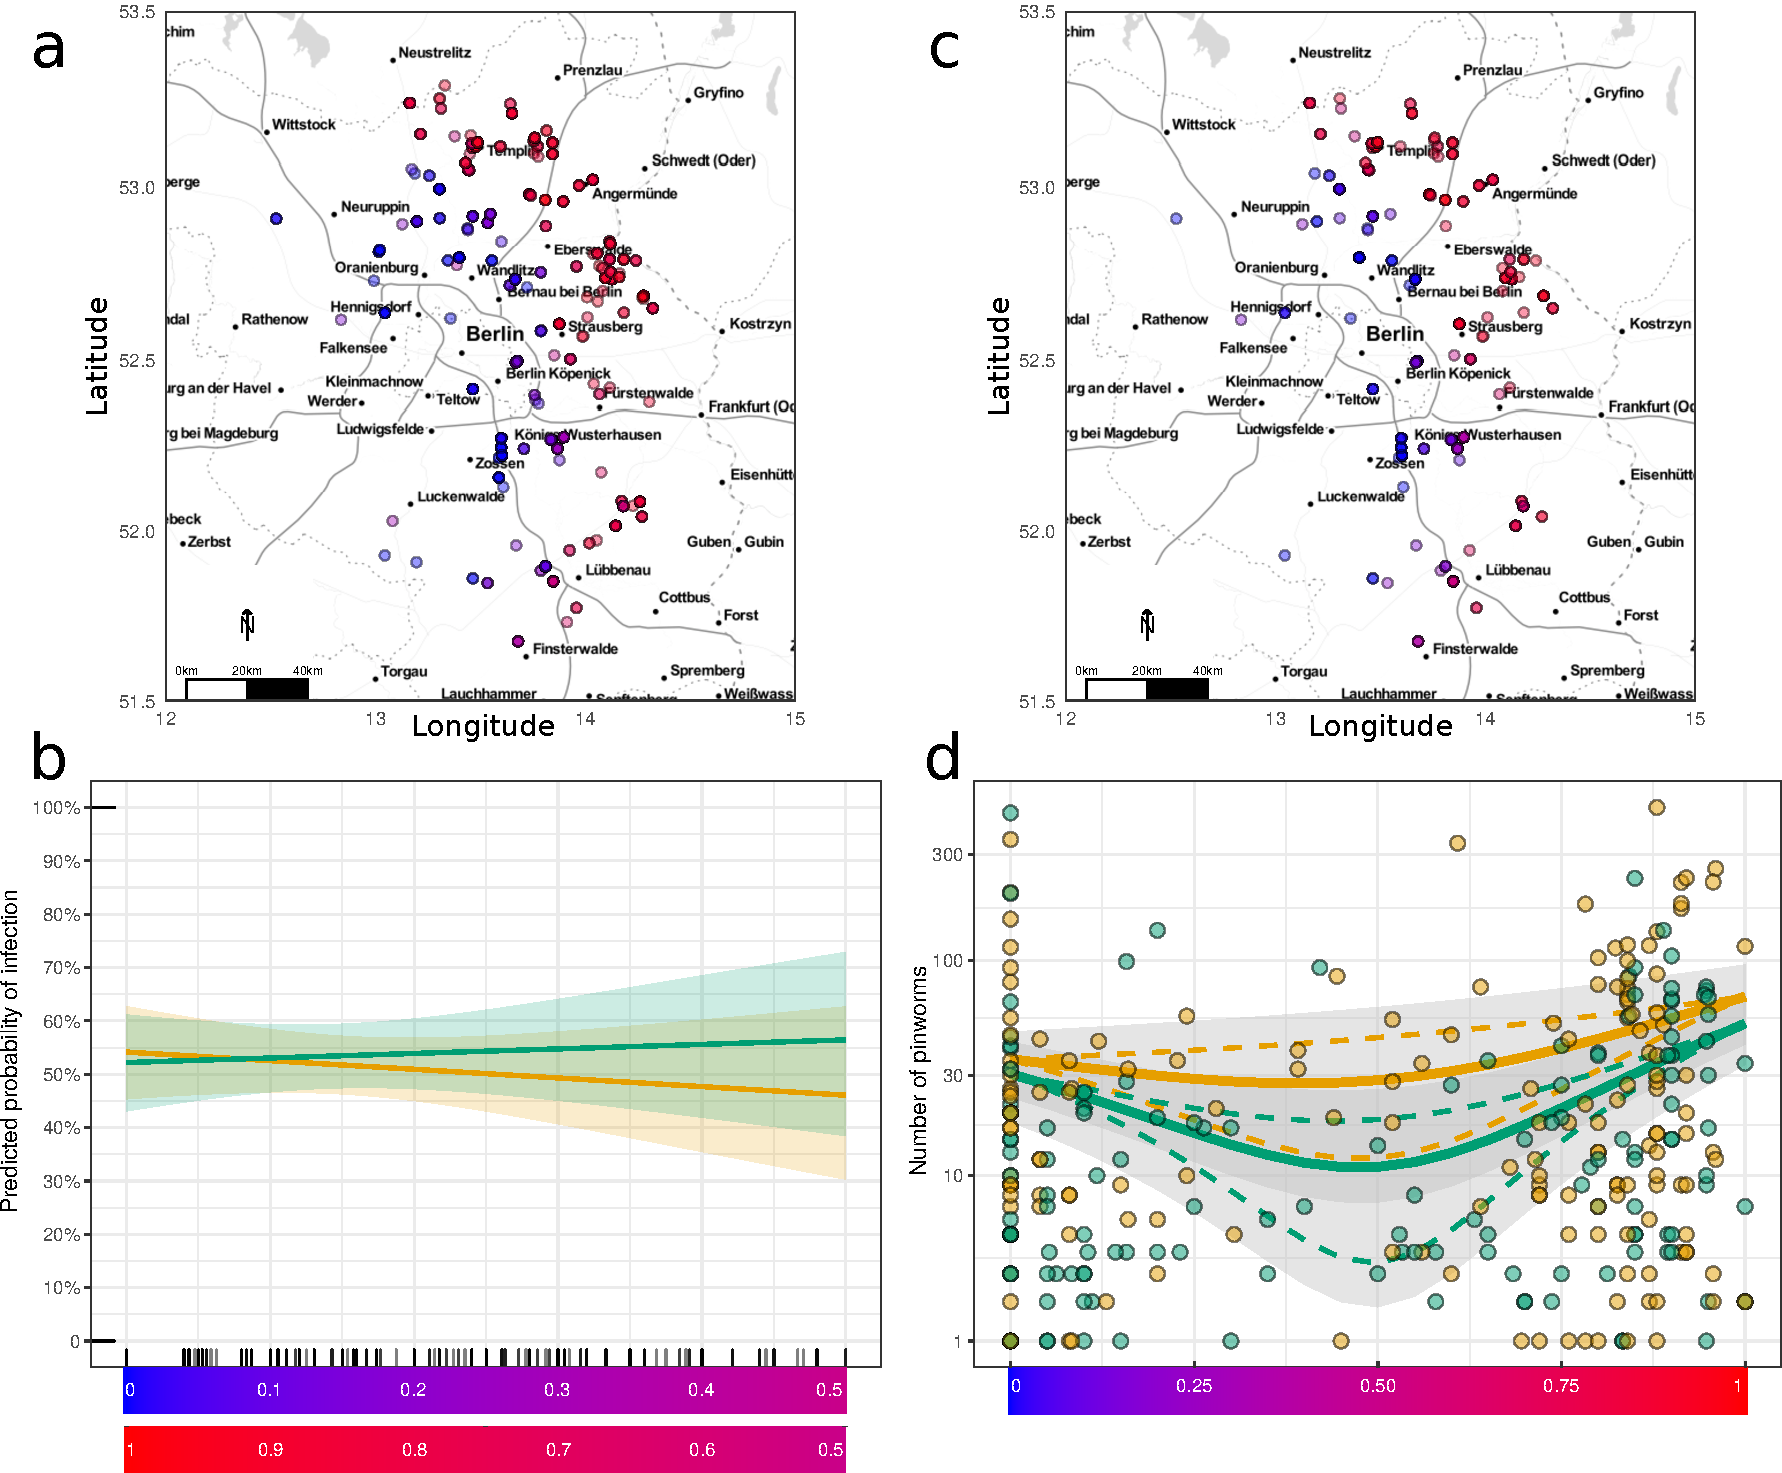
\includegraphics[scale=0.7]{Figure3.pdf}
      \end{tikzfigure} 

\end{multicols*}

\begin{itemize}
\item Equal parasite prevalence along the hybrid index
\item Statistically significant lower parasite load in the center of the hybrid zone
\item No indication of differential body condition between infected/non-infected / along hybrid gradient
\end{itemize}
\vfill\null \columnbreak
      

      
\Large \centering Body condition
      \begin{tikzfigure}[]
        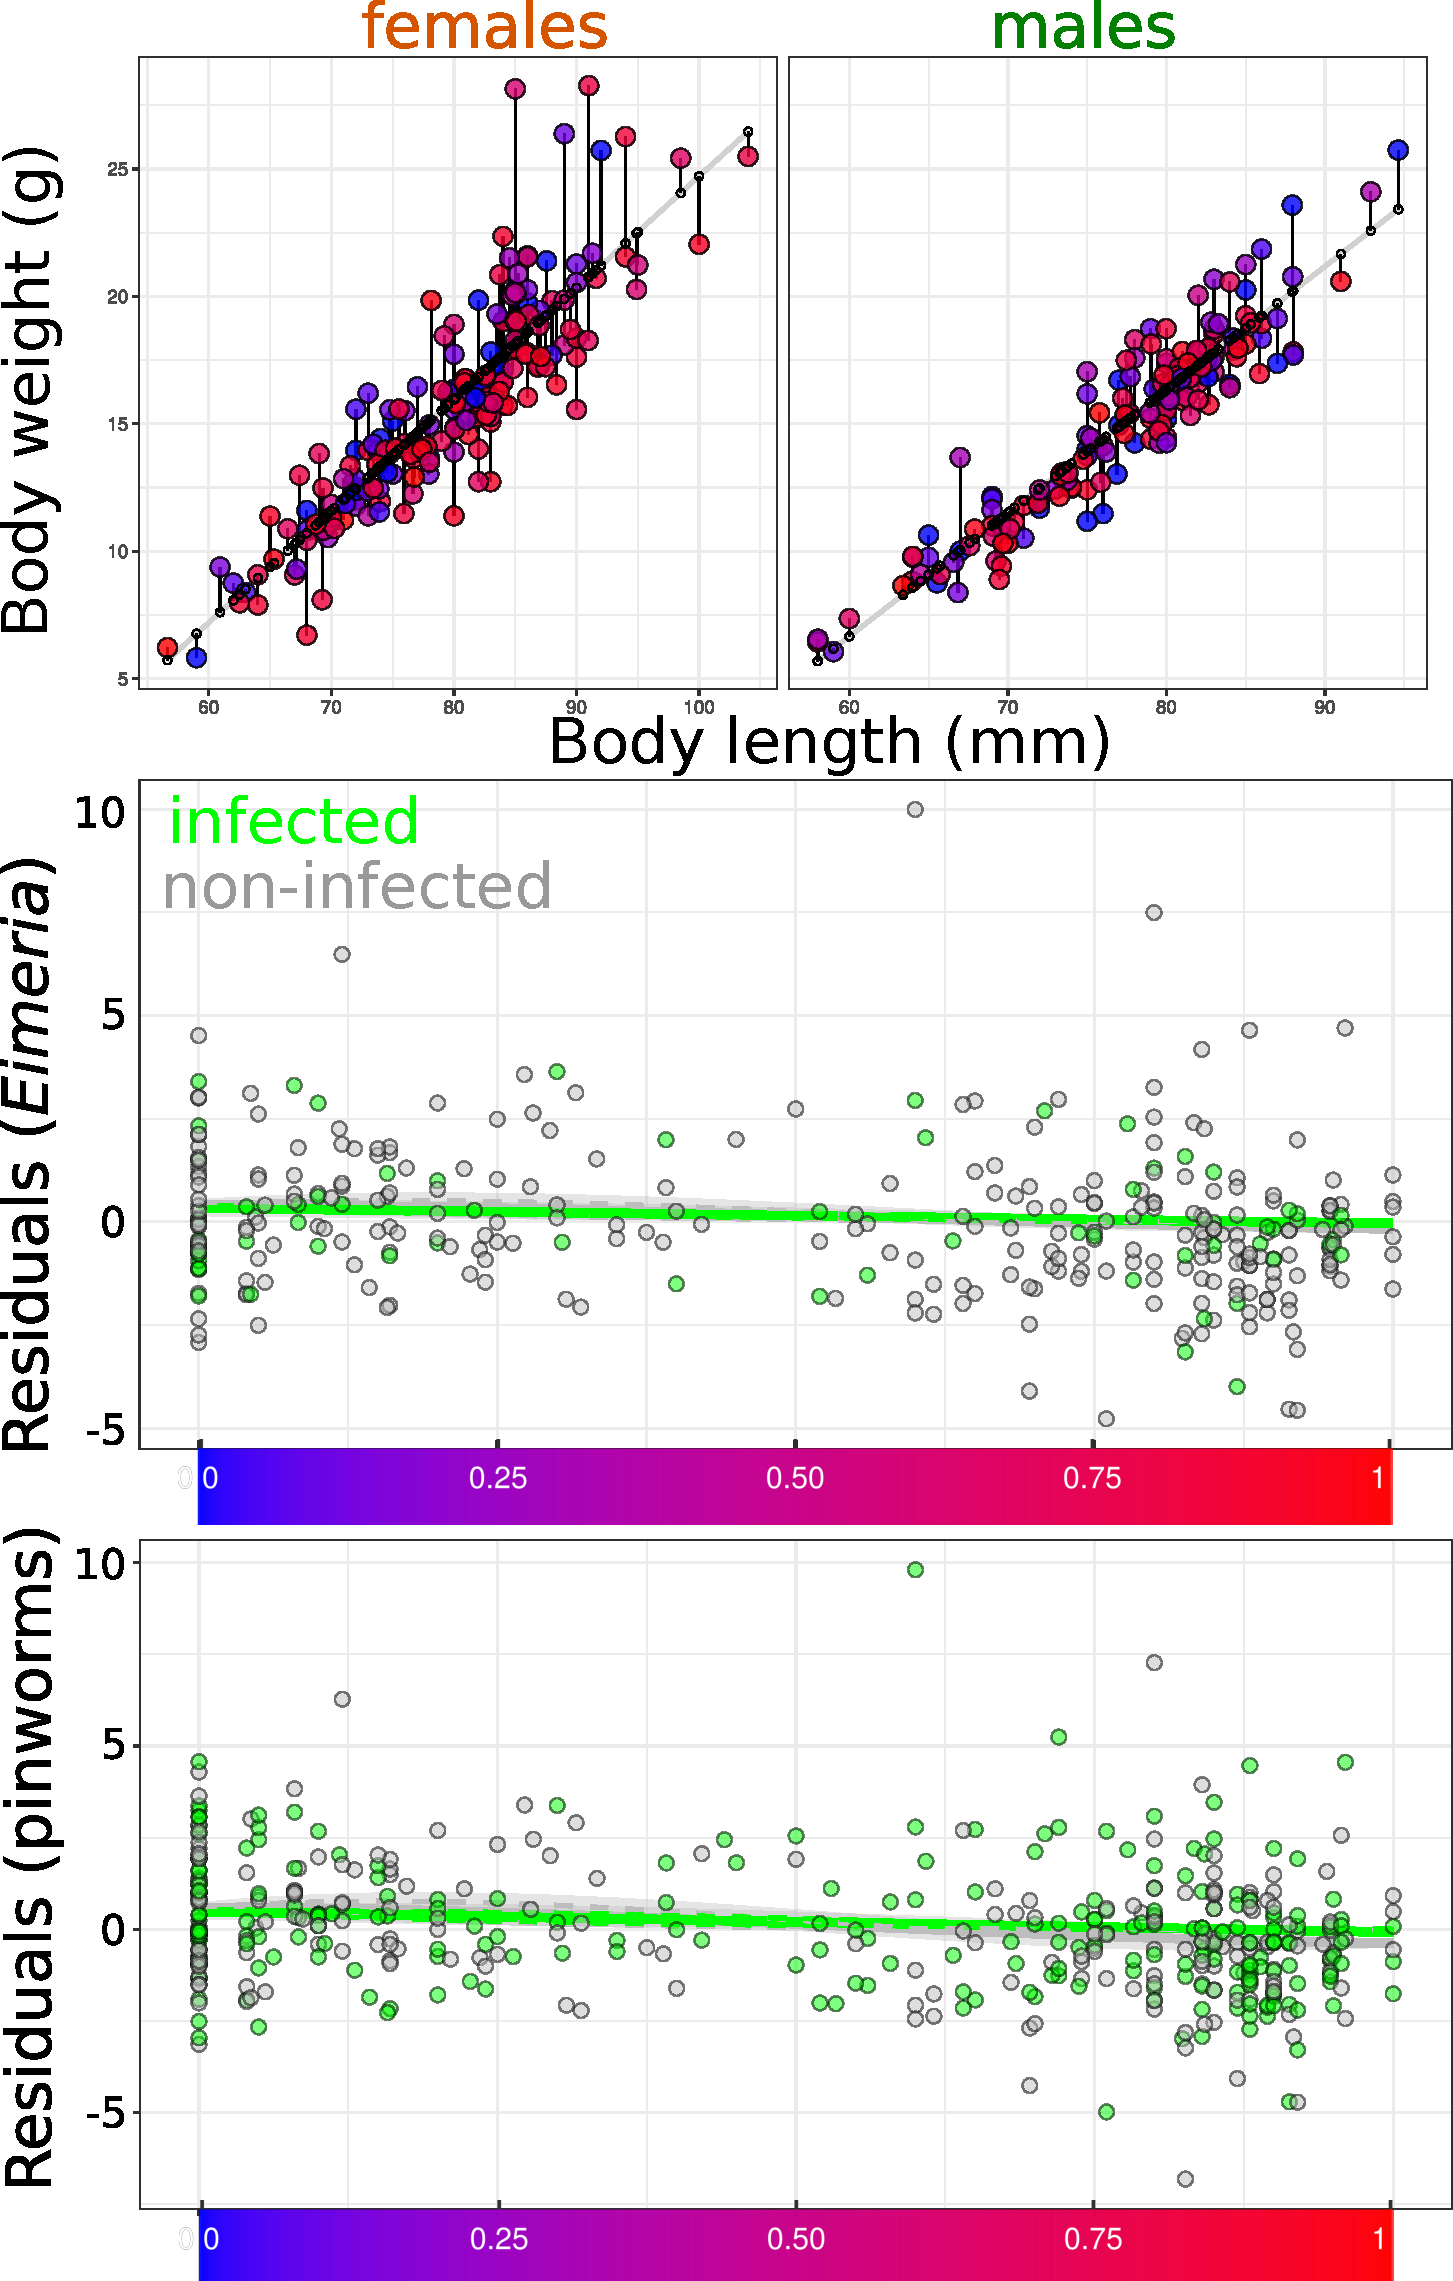
\includegraphics[scale=0.7]{Figure4.pdf}
      \end{tikzfigure}

      \end{multicols*}
      
%       \begin{multicols*}{2}
% 
% \begin{itemize}
% \item Equal parasite prevalence along the hybrid index
% \item Statistically significant lower parasite load in the center of the hybrid zone
% \item No indication of differential body condition between infected/non-infected / along hybrid gradient
% \end{itemize} \vfill\null \columnbreak
% 
% \end{multicols*}
}

\block{Conclusion}
{

\begin{itemize}
  \item Increased resistance of hybrid mice compared to parental strains for both lower pathogenic parasite (pinworms) and high pathogenic one (\textit{Eimeria})
  \item Control for density troughs: no evidence of a lower parasite prevalence in the centre of the hybrid zone (exclude external ecological epidemiological factors)
  \item \textbf{Independance} of hybrid resistance from the parasite pathogenicity level
  
\end{itemize}
}

% REFERENCES
% ----------


\begin{columns} 
  \column{0.7} \block{References}{
Balard \textit{et al.} (unpublished) Reduced \textit{Eimeria} and pinworms loads in hybrid mice of the European house mouse hybrid zone \newline
R package used for modelling: Balard, A., and E. Heitlinger. 2019. Alicebalard/parasiteLoad DOI: 10.5281/zenodo.2535547
  }
  \column{0.3} \block{}{
    \begin{tikzfigure}[]
      
\includegraphics[scale=0.8]{AllLogos.png}
    \end{tikzfigure}}
\end{columns}

% ----------------
\end{document}
\endinput
%%
%% End of file 
